\subsection[Генераторы с несколькими регистрами сдвига]{Генераторы с несколькими регистрами \protect\\ сдвига}
\selectlanguage{russian}

Первый способ улучшения криптографических свойств последовательности состоит в создании композиционных генераторов из нескольких регистров сдвига при определенном способе выбора параметров. Схема такого генератора показана на рис. \ref{fig:generators}. Здесь $L_i, ~ i = 1, 2, \dots, M$ -- регистры сдвига с линейной обратной связью. Вырабатываемые ими двоичные символы $x_{1,i}, x_{2,i},  \dots, x_{M,i}$ поступают синхронно на устройство преобразования, задаваемое булевой функцией $f(x_{1,i}, x_{2,i}, \dots, x_{M,i})$. В булевой функции аргументы принимают значения $0,1$ и значения функции также $0,1$.

Число ячеек в $i$-м регистре равно $L_{i}$, причем $\gcd(L_i, L_j)=1$ для $i \neq j$, где  $\gcd$ -- наибольший общий делитель. Общее число ячеек $L = \sum\limits_{i=1}^M L_i$. Булева функция $f$ должна включать слагаемое по одному из входов, т.~е. $f = \dots + x_i + \dots$, для того, чтобы двоичные символы на выходе этой функции были равновероятными. Период этого генератора может достигать величины (немного меньше)
    \[ T \simeq 2^L. \]

\begin{figure}[!ht]
	\centering
	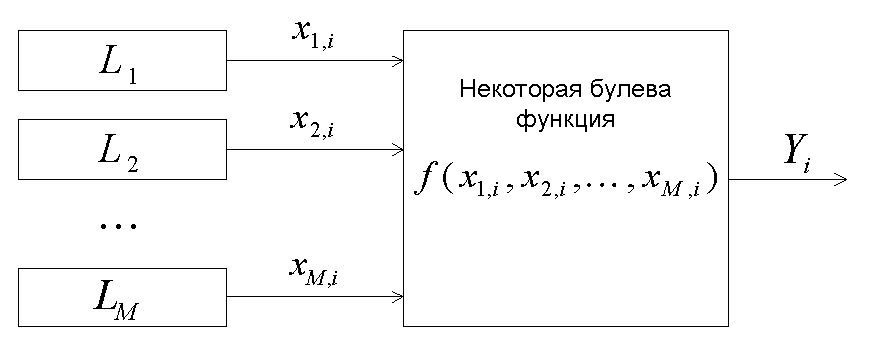
\includegraphics[width=0.7\textwidth]{pic/generators}
    \caption{Генератор с несколькими регистрами сдвига\label{fig:generators}}
\end{figure}

Таким образом, увеличение числа регистров сдвига с обратной связью увеличивает период последовательности. Однако более важным параметром для увеличения криптостойкости генератора является \emph{ длина регистра с линейной обратной связью}, эквивалентного по порождаемой последовательности. Такой эквивалентный регистр с линейной обратной связью находится с помощью алгоритма Берлекэмпа~---~Мэсси декодирования циклических кодов. В лучшем случае длина эквивалентного регистра соизмерима с периодом последовательности, порожденной нелинейным генератором. В общем случае определение эквивалентной длины является сложной задачей.
